%Einrücken bei Absatz verhindern
\setlength{\parindent}{0em} 

%**********************************************************************************
% Kapitel Maßnahmen und Qualitätsüberprüfung
%**********************************************************************************
\chapter{Qualitätsüberprüfung}
\section{Validierung der umgesetzten Maßnahmen}
In den vorangegangenen Kapitel wurden Maßnahmen zur Umsetzung von technischen IT-Sicherheitsanforderungen an eine Bank in Österreich untersucht. Die Frage die sich stellt ist, wie eine erfolgreiche Umsetzung dieser Maßnahmen gemessen und in weiterer Folge auditiert werden kann. 
\bigbreak
Im Zuge der Ausarbeitung haben sich folgende Möglichkeiten für die Überprüfung einer korrekten Umsetzung ergeben:
\begin{itemize}
    \item Technische Überprüfung
    \begin{itemize}
        \item Überprüfung durch interne Mechanismen\\
        Einige Produkte, mit denen Maßnahmen umgesetzt werden, bieten die Möglichkeit interner Kontrollmechanismen um die ordnungsgemäße Funktionalität des Produktes sicherzustellen. So bieten Identity-Management Systeme etwa die Möglichkeit zur Rezertifizierung von Berechtigungen oder zur Analyse ob nicht korrelierte Accounts bestehen. Auf Basis dieser Mechanismen können regelmäßige Kontrollen etabliert und auditiert werden. 
        \item Überprüfung mittels Penetration-Test\\
        Umgesetzte IT-Sicherheitsanforderungen lassen sich häufig mittels Penetration-Test überprüfen. Auf Basis unterschiedlicher Penetration-Tests, wie in Kapitel \ref{ch:penetration-tests} beschrieben, können Angriffe simuliert und die Funktionalität der IT-Sicherheitsmaßnahme überprüft werden.
        \item Überprüfung mittels Katastrophentest oder \glqq{}Business-Continuity Management\grqq{} (BCM)\\
        Ähnlich wie bei Penetration-Tests lassen sich umgesetzte Maßnahmen im Zuge eines Katastrophentests überprüfen. Häufig decken Bereiche aus dem BCM auch IT-Sicherheitsmaßnahmen ab. Im Zuge eines Katastrophentests können die Ausfallsicherheit von Systemen oder die einwandfreie Funktionalität von Backup-Prozessen überprüft werden. 
    \end{itemize}
    \item Organisatorische Überprüfung
    \begin{itemize}
        \item Überprüfung mittels Audits\\
        Interne und externe Audits sind das erste Mittel der Wahl um die Umsetzung von technischen IT-Sicherheitsmaßnahmen und deren korrekte Arbeitsweise sicherzustellen. 
        \item Überprüfung mittels internem Kontrollsystem (IKS)\\
        Auch mittels eines IKS kann die Umsetzung von Maßnahmen überprüft werden. Im Falle von Firewall-Änderungen etwa können beispielsweise periodisch Stichproben genommen und die Legitimität der Änderungen überprüft werden. 
        \item Überprüfung mittels Service-Level Agreement (SLA)\\
        Mittels vereinbarter SLAs lässt sich nicht nur die Funktionalität sondern auch die Effizienz von umgesetzten Maßnahmen überprüfen. So können SLAs Auskunft darüber geben ob kritische System-Patchens eingespielt werden und wie viel Zeit das Update in Anspruch nimmt.
    \end{itemize}
\end{itemize}
\bigbreak
Abbildung \ref{fig:matrix_ueberpruefung} zeigt die in Kapitel \ref{kap_anforderungsmatrix_abgleitete_maßnahmen} abgeleiteten IT-Sicherheitsmaßnahmen und passende Überprüfungsmethoden. 

\begin{figure}[H]
    \centering
  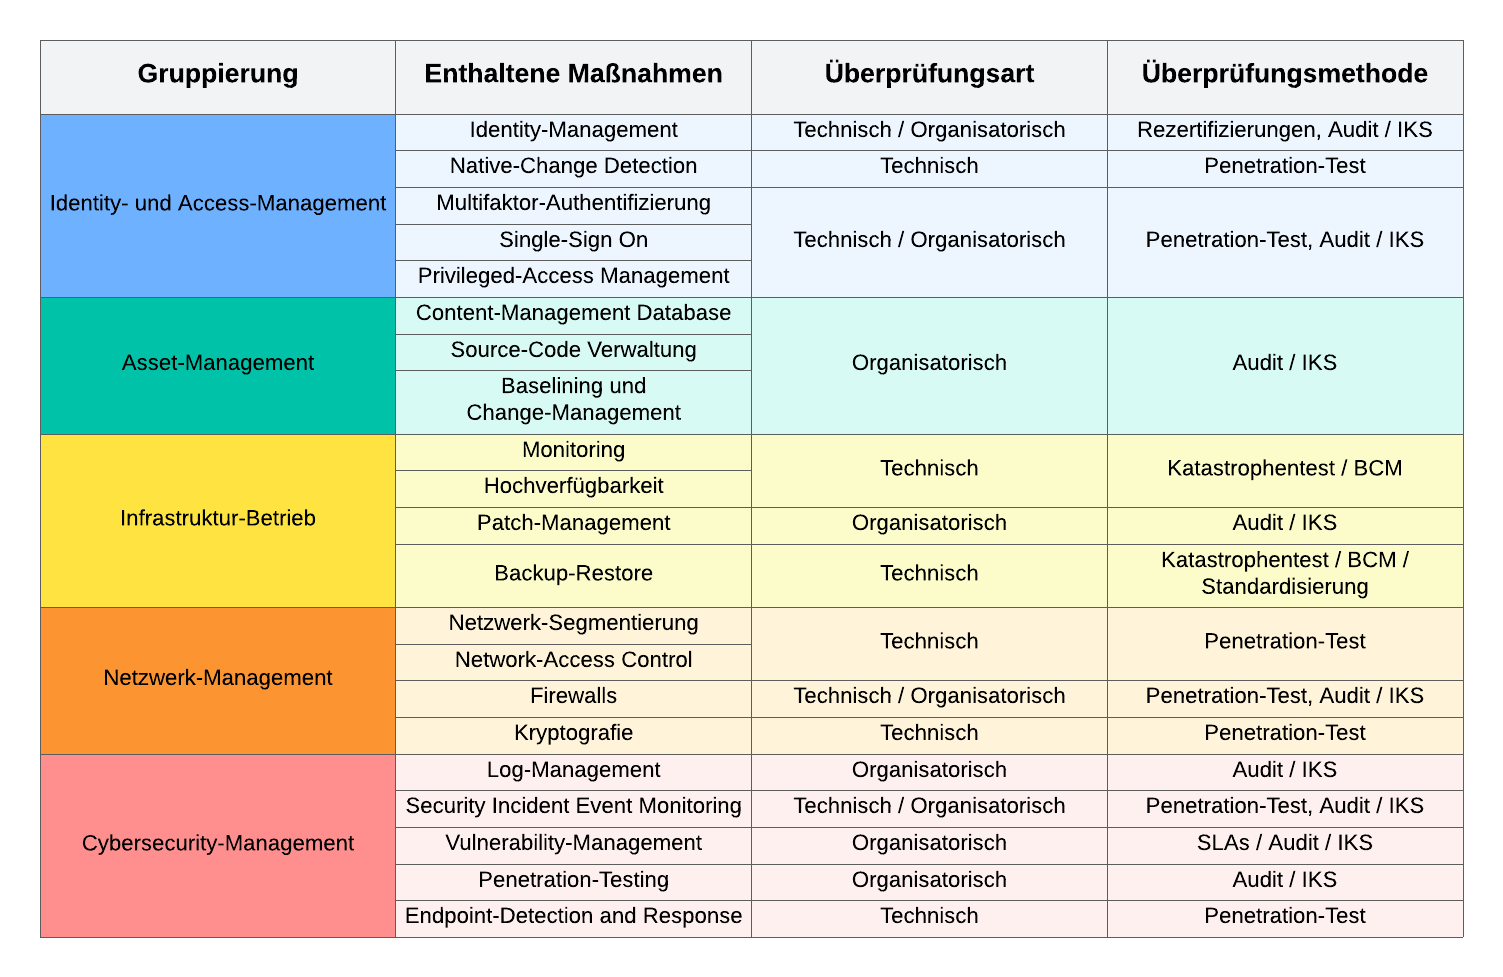
\includegraphics[width=\linewidth]{images/uploads/a_figure_16.png}
  \caption{Visuelle Darstellung der Gruppierung, enthaltenen Maßnahmen und Möglichkeit zur Überprüfung der Umsetzung. Quelle: Eigene Darstellung, 2022}
  \label{fig:matrix_ueberpruefung}
\end{figure}

\section{Vollständigkeit der Maßnahmen}
In Kapitel \ref{cha:Auswertung} wurden Maßnahmen und Best-Practice-Ansätze zur Umsetzung von technischen IT-Sicherheitsanforderungen an eine Bank in Österreich definiert und beschrieben. Zur Überprüfung, ob diese geeignet sind die Anforderungen der Aufsichtsbehörden zu erfüllen, werden die Maßnahmen und Best-Practice-Ansätze auf die \glqq{}OWASP Cyber Defense Matrix\grqq{} (CDM) angewandt \autocite{owasp_cyber_defense_matrix}. 
\bigbreak

Die CDM ist ein Open-Source-Community-Projekt unter der Leitung der OWASP\footnote{https://owasp.org} und in Abbildung \ref{fig:OWASP-CDM} dargestellt. Es handelt sich um eine zweidimensionale Matrix mit den fünf Kernfunktionen des \glqq{}NIST Cybersecurity Frameworks\grqq{} auf der X-Achse und fünf unterschiedlichen Asset-Ausprägungen auf der Y-Achse \autocite{NIST_Cybersec_Framework}. 
Das \glqq{}Nation Institute of Standards and Technology\grqq{} (NIST\footnote{https://www.nist.gov}) definiert fünf grundlegende Kernfunktionen zur Behandlung von- und zum Schutz vor Cyberangriffen, zu sehen in Abbildung \ref{fig:NIST-Framework}. 
\bigbreak
Die fünf Kernfunktionen beziehen sich auf die Zeit vor und nach einem erfolgreichen Angriff \autocite{NIST}:
\begin{itemize}
    \item Pre-incident:
    \begin{itemize}
        \item Identify\\
        Identifizierung der im Unternehmen befindlichen Assets.
        \item Protect\\
        Schutz aller im Unternehmen befindlichen Assets und/oder die Etablierung von mitigierenden Maßnahmen.
    \end{itemize}
    \item Post-incident:
    \begin{itemize}
        \item Detect\\
        Erkennen von schadhaften Aktivität auf den Assets.
        \item Respond\\
        Reaktion auf schadhafte Aktivitäten auf den Assets.
        \item Recover\\
        Wiederherstellung der jeweiligen Assets.
    \end{itemize}
\end{itemize}
\bigbreak
Die Y-Achse der CDM beschreibt fünf schützenswerte Ausprägungen von IT-Assets:
\begin{itemize}
    \item Devices\\
    Clients, Server, Storage, ...
    \item Applications\\
    Software Interaktion auf den Devices.
    \item Networks\\
    Client/Server Interaktionen, Daten die über das Netzwerk übertragen werden.
    \item Data\\
    Daten die auf den Devices gespeichert oder von diesen verarbeitet werden.
    \item Users\\
    Anwender der jeweiligen Assets.
\end{itemize}
\bigbreak
Der untere Bereich der Matrix zeigt eine Kombination aus benötigter Technologie, Menschen und relevanter Prozesse für die Adressierung der fünf Kernfunktionen. Es ist erkennbar, dass die Funktionen im linken Bereich der Matrix stark automatisiert mittels Technologie durchgeführt werden können. Die Funktionen im rechten Bereich der Matrix benötigen die Unterstützung durch Mitarbeiter und manuelles Doing. Etablierte und funktionierende Prozesse sind für alle fünf Kernfunktionen nötig.
\bigbreak
\begin{figure}[H]
    \centering
  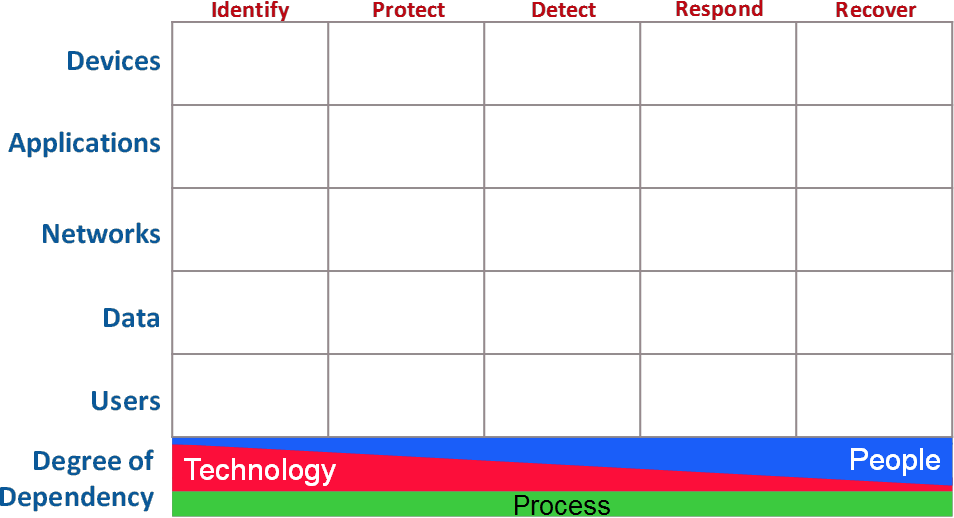
\includegraphics[width=\linewidth]{images/uploads/a_figure_12.png}
  \caption{Darstellung der CDM. Quelle: \textcite{owasp-CDM}, 2022}
  \label{fig:OWASP-CDM}
\end{figure}

\begin{figure}[H]
    \centering
  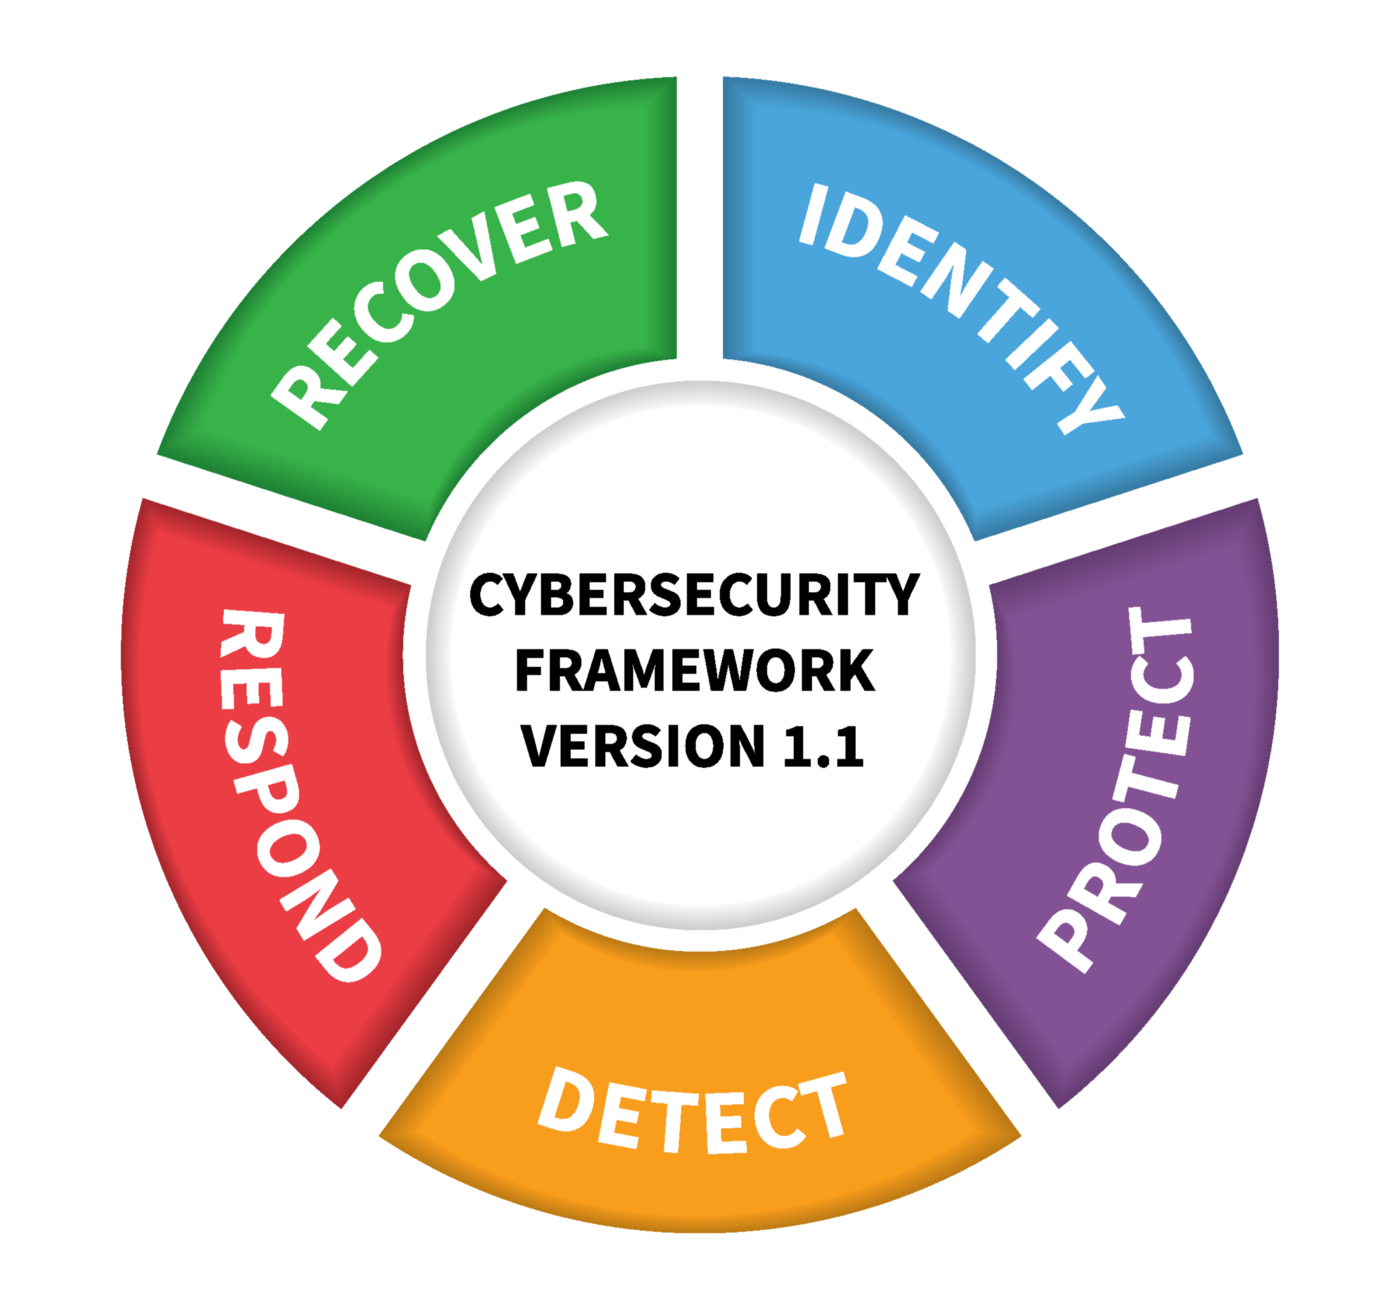
\includegraphics[scale=0.1]{images/uploads/a_figure_11.png}
  \caption{Darstellung der fünf Kernfunktionen des NIST Cybersecurity Frameworks. Quelle: \textcite{NIST}, 2022}
  \label{fig:NIST-Framework}
\end{figure}
\bigbreak
Im Zuge der Qualitätsüberprüfung werden die in Kapitel \ref{cha:Auswertung} definierten IT-Sicherheitsmaßnahmen und Best-Practice-Ansätze in die CDM eingetragen. Hierfür ist relevant in welcher Angriffsphase, welche Ausprägung von IT-Asset, mit Hilfe der jeweiligen Maßnahme geschützt werden. Dieser Vorgang lässt sich am Beispiel IAM verdeutlichen. Mit Hilfe von IAM können Anwender im Unternehmen eindeutig identifiziert werden. Des Weiteren bietet IAM Mechanismen zum Schutz der Anwender, etwa vor unerlaubter Verwendung von Benutzerdaten. Auch eine unerlaubte Verwendung von Benutzerdaten kann mittels IAM erkannt werden. Aus diesem Grund ist die Maßnahme IAM in der CDM in den Bereichen \glqq{}Users - Identify\grqq{}, \glqq{}Users - Protect\grqq{} und \glqq{}Users - Detect\grqq{} zu finden. 
\bigbreak
Es ist zu erkennen, dass die abgeleiteten Maßnahmen und Best-Practice-Ansätze einen Großteil der fünf Kernfunktionen der Matrix adressieren. Im Zuge der Ausarbeitung hat sich herausgestellt, dass die Punkte \glqq{}Identify Data\grqq{}, \glqq{}Respond Users\grqq{} und \glqq{}Recover Users\grqq{} technisch nicht realisierbar sind. Eine Identifizierung und Klassifizierung der in einem Unternehmen verwendeten Daten benötigen eine manuelle Betrachtung und kann nicht technisch realisiert werden. Die Punkte \glqq{}Detect Data\grqq{} und \glqq{}Respond Data\grqq{} wurden in den Anforderungen in Kapitel \ref{cha:regulatorische_anforderungen_und_vorgaben} und daher auch in den umzusetzenden Maßnahmen in Kapitel \ref{kap_anforderungsmatrix_abgleitete_maßnahmen} nicht betrachtet. Eine mögliche Maßnahme für \glqq{}Detect Data\grqq{} bietet die Recherche nach unternehmensrelevanten Daten im Darknet. Ein Beispiel für den Bereich \glqq{}Respond Data\grqq{} liefert die Implementierung von \glqq{}Digital Rights Management\grqq{}, der Kontrolle und dem Management von urheberrechtlich geschützten Daten. 
\bigbreak
Abbildung \ref{fig:CDM-self} zeigt die CDM, mit den in Kapitel \ref{kap_anforderungsmatrix_abgleitete_maßnahmen} abgeleiteten Maßnahmen und den in Kapitel \ref{cha:Auswertung} definierten Best-Practice-Ansätzen.  

\begin{figure}[H]
    \centering
 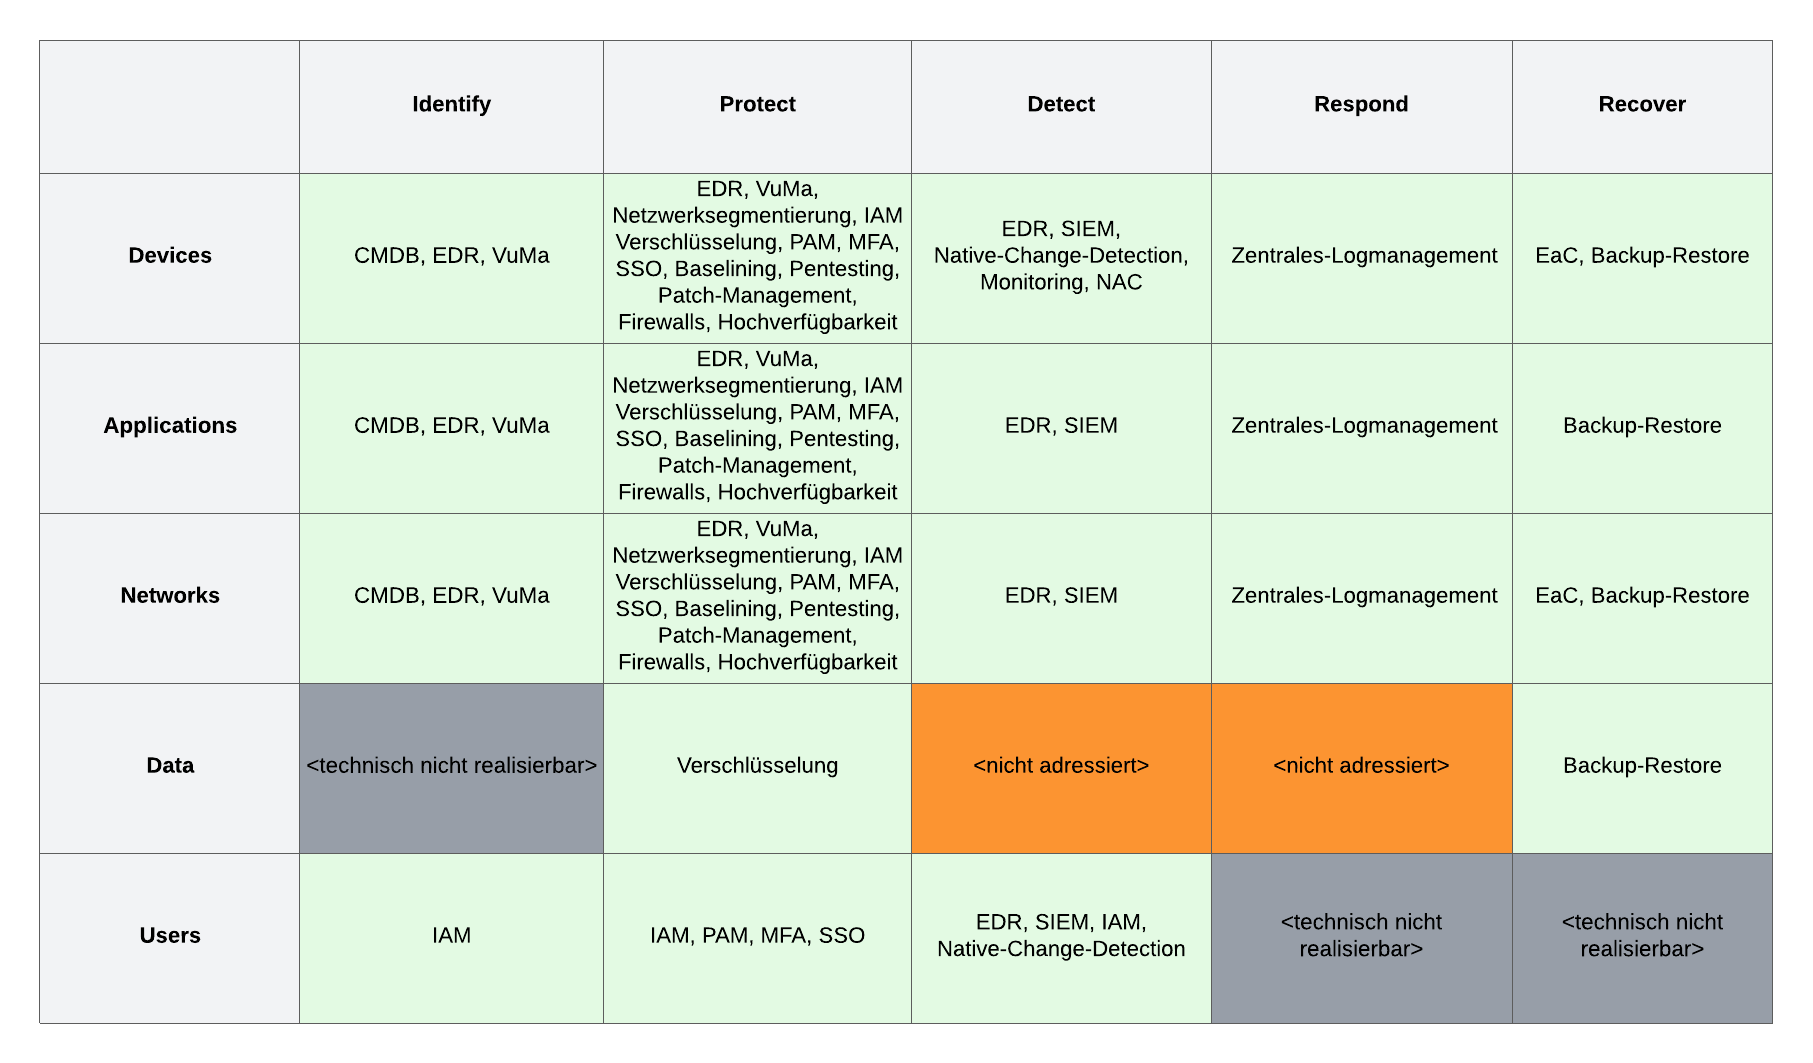
\includegraphics[width=\linewidth]{images/uploads/a_figure_14.png}
  \caption{Darstellung der CDM mit den definierten Best-Practice-Ansätzen und damit einhergehenden Maßnahmen. Quelle: Eigene Darstellung, 2022}
  \label{fig:CDM-self}
\end{figure}
\bigbreak